 \section{Unidad 1}
       \subsection{Cálculos numéricos}
%
      \ejemplosboxed[5]{Realiza las siguientes operaciones de \textit{cálculo numérico}:

		\begin{parts}
			\begin{multicols}{2}

				% \addcontentsline{toc}{subsection}{Suma de números}
				% \subsubsection*{Suma de números}
				
			%	\part $849.332+242.25+469.381=$ \fillin[$1560.963$][0in]
				
				%\part $27.05+34.99+0.1=$ \fillin[$62.14$][0in]
				
				\part $0.1+0.02+0.03+0.4=$ \fillin[$0.55$][0in]
				
			%	\part $0.11+2+3.8=$ \fillin[$5.91$][0in]

				% \addcontentsline{toc}{subsection}{Resta de números}
				% \subsubsection*{Resta de números}
				
			%	\part $4934-451-682=$ \fillin[$3801$][0in]
				
			%	\part $0.1-0.02=$ \fillin[$0.08$][0in]
				
				\part $0.1-0.02-0.03-0.4=$ \fillin[$-0.35$][0in]
				
			%	\part $0.11-2-3.8=$ \fillin[$-5.69$][0in]

				% \addcontentsline{toc}{subsection}{Multiplicación de números}
				% \subsubsection*{Multiplicación de números}
				
				%\part $19.3\times6.27=$ \fillin[$121.011$][0in]
				
				\part $0.1\times0.02=$ \fillin[$0.002$][0in]
				
				%\part $100.1\times 0.99=$ \fillin[$99.099$][0in]
				
				%\part $0.11\times2\times3.8=$ \fillin[$0.836$][0in]

				% \addcontentsline{toc}{subsection}{División de números}
				% \subsubsection*{División de números}
				
				\part $922\divisionsymbol1.2=$ \fillin[$768.333$][0in]
				
			%	\part $0.1\divisionsymbol0.02=$ \fillin[$5$][0in]
				
			%	\part $180\divisionsymbol 0.09=$ \fillin[$2000$][0in]
				
			%	\part $25.25\divisionsymbol 0.5=$ \fillin[$50.5$][0in]

				% \addcontentsline{toc}{subsection}{Resolución de problemas}

                                                \columnbreak%

                        % \subsubsection*{Resolución de problemas}

				\part Una computadora tiene un disco duro de 368 GB de memoria, si varios programas ocupan 128.75 GB. ¿Qué cantidad de memoria está libre?

				\begin{solutionbox}{1.2cm}
					$368-128.75=$ \fillin[$239.25$][0in]
				\end{solutionbox}
				
			\end{multicols}
		\end{parts}
      }

        \questionboxed[4]{Realiza las siguientes operaciones de \textit{cálculo numérico}:
           
      \begin{parts}
                  \begin{multicols}{2}
                        \subsubsection{Suma de números}
                        \part $\dfrac{5}{6}+\dfrac{3}{8}=$ \fillin[$1\dfrac{5}{24}$][0in]
                        \part $0.5+0.25+0.125=$ \fillin[$0.875$][0in]
                        \part $\dfrac{1}{2}+\dfrac{2}{5}=$ \fillin[$\dfrac{9}{10}$][0in]
                        \part $1.25+0.5+0.25=$ \fillin[$2$][0in]
                        \subsubsection{Multiplicación de números}
                        \part $9.27\times 5.4=$ \fillin[$50.058$][0in]
                        \part $0.5\times 0.25=$ \fillin[$0.125$][0in]
                        \part $0.5\times 0.25\times 0.125=$ \fillin[$0.015625$][0in]
                        \part $2.5\times 0.4=$ \fillin[$1$][0in]
                        \subsubsection{Resta de números}
                        \part $\dfrac{1}{2}-\dfrac{2}{5}=$ \fillin[$\dfrac{1}{10}$][0in]
                        \part $1.25-0.5-0.25=$ \fillin[$0.5$][0in]
                        \part $\dfrac{5}{6}-\dfrac{3}{4}=$ \fillin[$-\dfrac{1}{12}$][0in]
                        \part $0.5-0.25-0.125=$ \fillin[$0.125$][0in]
                        \subsubsection{División de números}
                        \part $622.21\divisionsymbol 115=$ \fillin[$5.41$][0in]
                        \part $0.5\divisionsymbol 0.25=$ \fillin[$2$][0in]
                        \part $5\divisionsymbol 0.5=$ \fillin[$10$][0in]
                        \part $\dfrac{1}{2}\divisionsymbol\dfrac{2}{5}=$ \fillin[$\dfrac{5}{4}$][0in]
                        \subsubsection{Resolución de problemas}
                        \part Si un dólar equivale a 19 pesos. ¿Cuántos dólares serán 1634 pesos? \fillin[$1634\divisionsymbol 19 =$ 86 dólares][0in]
                        % \part Los alumnos de secundaria van a comprar un balón de fútbol que cuesta 437.50 pesos. Si son un total de 35 alumnos, ¿con cuánto dinero debe cooperar cada alumno? \fillin[$437.50\divisionsymbol 35 =$ 12.5 pesos][0in]
                        \part Un automóvil viaja a 112.4 kilómetros por hora en una carretera. ¿Qué distancia recorre en 4 horas? \fillin[$112.4\times 4 =$ 449.6 kilómetros][0in]
                  \end{multicols}
            \end{parts}
      }

      \subsection{Leyes de los exponentes}
    
       \ejemplosboxed[9]{Realiza las siguientes operaciones con exponentes:
            
      \begin{multicols}{3}
                  \begin{parts}
                        % \addcontentsline{toc}{subsection}{Suma de exponentes}
	\subsubsection{Suma de exponentes}
             
      \part $(-5a^4)(-3a^2)=$
                       
                        \begin{solutionbox}{1.2cm}
                              $(-5a^4)(-3a^2) = 15a^6$
                        \end{solutionbox}

                        \part $(-3a^4)(8a^2)=$
                      
                        \begin{solutionbox}{1.2cm}
                              $(-3a^4)(8a^2) = -24a^6$
                        \end{solutionbox}

                        \part $4x^2\cdot x^5\cdot 5x^8=$
                      
                        \begin{solutionbox}{1.2cm}
                              $4x^2\cdot x^5\cdot 5x^8 = 20x^{15}$
                        \end{solutionbox}

                        \part $x^2y^3z^4 \cdot x^5z^4=$
                     
                        \begin{solutionbox}{1.2cm}
                              $x^2y^3z^4 \cdot x^5z^4 = x^7y^3z^8$
                        \end{solutionbox}

                        \columnbreak

                        \part $x^3x^2x^3=$
                     
                        \begin{solutionbox}{0.8cm}
                              $x^3x^2x^3 = x^8$
                        \end{solutionbox}

                        \part $7x^2\cdot 3x^4 \cdot 6x^2=$
                     
                        \begin{solutionbox}{1.2cm}
                              $7x^2\cdot 3x^4 \cdot 6x^2 = 126x^8$
                        \end{solutionbox}

                        % \addcontentsline{toc}{subsection}{Resta de exponentes}
	\subsubsection{Resta de exponentes}
                        
      \part $\dfrac{x^{13}y^{18}z^{4}}{x^{11}y^{9}z^{4}}=$
                     
                        \begin{solutionbox}{1.5cm}
                              $\dfrac{x^{13}y^{18}z^{4}}{x^{11}y^{9}z^{4}} = x^2y^9$
                        \end{solutionbox}

                        \part $\dfrac{x^{4}y^{12}z^{13}}{x^{3}y^{12}z^{13}}=$
                    
                        \begin{solutionbox}{1cm}
                              $\dfrac{x^{4}y^{12}z^{13}}{x^{3}y^{12}z^{13}} = x$
                        \end{solutionbox}

                        \part $\dfrac{81a^5b^{12}c^9}{9a^3b^{7}c^5}=$
                     
                        \begin{solutionbox}{1.2cm}
                              $\dfrac{81a^5b^{12}c^9}{9a^3b^{7}c^5} = 9a^2b^5c^4$
                        \end{solutionbox}

                        % \addcontentsline{toc}{subsection}{Multiplicación de exponentes}
	\subsubsection{Multiplicación de exponentes}
                       
                        \part $(a^3b^2c^4)^3=$
                     
                        \begin{solutionbox}{1cm}
                              $(a^3b^2c^4)^3 = a^9b^6c^{12}$
                        \end{solutionbox}

                        \part $\left(x^4 y^5\right)^6=$
                    
                        \begin{solutionbox}{1.2cm}
                              $\left(x^4 y^5\right)^6 = x^{24}y^{30}$
                        \end{solutionbox}

                        \part $\left(a^3 b^5 c^{11} \right)^7=$
                  
                        \begin{solutionbox}{1.2cm}
                              $\left(a^3 b^5 c^{11} \right)^7 = a^{21}b^{35}c^{77}$
                        \end{solutionbox}
                  \end{parts}
            \end{multicols}
      }

      % \subsubsection{Suma de exponentes}

      %   \ejemplosboxed[2]{Realiza las siguientes operaciones con exponentes:

	% 	\begin{multicols}{2}
	% 		\begin{parts}
				
	% 			% \part $(2a^3)(-a)=$%\fillin[$-2a^4$][0in]

	% 			% \begin{solutionbox}{1cm}
	% 			% 	$(2a^3)(-a)= -2a^4$
	% 			% \end{solutionbox}

	% 			% \part $(5y^5)(7y^4)=$  %\fillin[$35y^9$][0in]

	% 			% \begin{solutionbox}{1cm}
	% 			% 	$(5y^5)(7y^4)=35y^9$
	% 			% \end{solutionbox}

	% 			\part $(-3a^4)(8a^2)=$ %\fillin[$-24a^6$][0in]

	% 			\begin{solutionbox}{0.8cm}
	% 				$(-3a^4)(8a^2) = -24a^6$
	% 			\end{solutionbox}

	% 			\part $3x^4\cdot 6x^7 \cdot 6x^2=$  %\fillin[$18x^{11}$][0in]

	% 			\begin{solutionbox}{0.8cm}
	% 				$3x^4\cdot 6x^7 \cdot 6x^2 = 108x^{13}$
	% 			\end{solutionbox}
	% 		\end{parts}
	% 	\end{multicols}
	% }

	\questionboxed[3]{Realiza las siguientes operaciones con exponentes:

		\begin{multicols}{3}
			\begin{parts}
				\part $(-5a^4)(-3a^2)=$ \fillin[$15a^6$][0in]\\

				% \begin{solutionbox}{1cm}
				% 	$(-5a^4)(-3a^2) = 15a^6$
				% \end{solutionbox}

				\part $(5x^3)(-x^{11})=$ \fillin[$-5x^{14}$][0in]\\

				% \begin{solutionbox}{1cm}
				% 	$(5x^3)(-x^{11})= -5x^{14}$
				% \end{solutionbox}

				\part $x^4x^{12}x^7=$ \fillin[$x^{23}$][0in]


				% \begin{solutionbox}{1cm}
				% 	$x^4x^{12}x^7= x^{23}$
				% \end{solutionbox}

				\part $(-2a^3)(-a)=$ \fillin[$-2a^4$][0in]\\

				% \begin{solutionbox}{1cm}
				% 	$(-2a^3)(-a)= -2a^4$
				% \end{solutionbox}

				\part $(5y^5)(7y^4)=$  \fillin[$35y^9$][0in]\\

				% \begin{solutionbox}{1cm}
				% 	$(5y^5)(7y^4)=35y^9$
				% \end{solutionbox}

				\part $(-3a^4)(8a^2)=$ \fillin[$-24a^6$][0in]

				% \begin{solutionbox}{1cm}
					% $(-3a^4)(8a^2) = -24a^6$
				% \end{solutionbox}

				\part $4x^2\cdot x^5\cdot 5x^8=$ \fillin[$20x^{15}$][0in]\\

				% \begin{solutionbox}{1cm}
				% 	$4x^2\cdot x^5\cdot 5x^8 = 20x^{15}$
				% \end{solutionbox}

				\part $x^2y^3z^4 \cdot x^5z^4=$ \fillin[$x^7y^3z^8$][0in]\\

				% \begin{solutionbox}{1cm}
				% 	$x^2y^3z^4 \cdot x^5z^4 = x^7y^3z^8$
				% \end{solutionbox}

				\part $7x^2\cdot 3x^4 \cdot 6x^2=$  \fillin[$126x^8$][0in]

				% \begin{solutionbox}{1cm}
				% 	$7x^2\cdot 3x^4 \cdot 6x^2 = 126x^8$
				% \end{solutionbox}
			\end{parts}
		\end{multicols}
	}

    


	% \subsubsection{Resta de exponentes}

	\questionboxed[4]{Realiza las siguientes operaciones con exponentes:

		\begin{multicols}{3}
			\begin{parts}
				\part $\dfrac{24x^{15}}{6x^{12}}=$ \fillin[$4x^3$][0in]\\

				% \begin{solutionbox}{1.5cm}
				% 	$\dfrac{18x^{15}}{6x^{12}}=3x^3$
				% \end{solutionbox}

				\part $\dfrac{6x^{7}}{2x^{2}}=$ \fillin[$3x^5$][0in]\\

				% \begin{solutionbox}{1.5cm}
				% 	$\dfrac{6x^{7}}{2x^{2}}=3x^5$
				% \end{solutionbox}

				\part $\dfrac{a^3b^{9}c^5}{a^2b^{5}c^4}=$ \fillin[$ab^4c$][0in]\\

				% \begin{solutionbox}{1.5cm}
				% 	$\dfrac{a^3b^{9}c^5}{a^2b^{5}c^4}=ab^4c$
				% \end{solutionbox}

				\part $\dfrac{x^{13}y^{18}z^{4}}{x^{11}y^{9}z^{4}}=$ \fillin[$x^2y^9$][0in]\\

				% \begin{solutionbox}{1.5cm}
				% 	$\dfrac{x^{13}y^{18}z^{4}}{x^{11}y^{9}z^{4}} = x^2y^9$
				% \end{solutionbox}

				\part $\dfrac{21x^{23}}{7x^{11}}=$ \fillin[$3x^{12}$][0in]\\

				% \begin{solutionbox}{1.5cm}
				% 	$\dfrac{21x^{23}}{7x^{11}}=3x^{12}$
				% \end{solutionbox}

				\part $\dfrac{25x^{8}}{5x^{3}}=$ \fillin[$5x^5$][0in]\\

				% \begin{solutionbox}{1.5cm}
				% 	 $\dfrac{25x^{8}}{5x^{3}}=5x^5$
				% \end{solutionbox}

				\part $\dfrac{x^{3}y^{12}z^{13}}{x^{3}y^{12}z^{13}}=$ \fillin[$1$][0in]\\

				% \begin{solutionbox}{1.5cm}
				% 	$\dfrac{x^{3}y^{12}z^{13}}{x^{3}y^{12}z^{13}} = 1$
				% \end{solutionbox}

				\part $\dfrac{81a^5b^{12}c^9}{9a^3b^{7}c^5}=$ \fillin[$9a^2b^5c^4$][0in]\\

				% \begin{solutionbox}{1.5cm}
				% 	$\dfrac{81a^5b^{12}c^9}{9a^3b^{7}c^5} = 9a^2b^5c^4$
				% \end{solutionbox}

				\part $\dfrac{5x^{8}}{25x^{3}}=$ \fillin[$\dfrac{x^5}{5}$][0in]

				% \begin{solutionbox}{1.5cm}
				% 	$\dfrac{5x^{8}}{25x^{3}}=\dfrac{x^5}{5}$
				% \end{solutionbox}
			\end{parts}
		\end{multicols}
	}	

	% \subsubsection{Multiplicación de exponentes}

	\questionboxed[4]{Realiza las siguientes operaciones con exponentes:

	\begin{multicols}{3}
		\begin{parts}
			\part $(a^3b^2c^4)^3=$ \fillin[$a^9b^6c^{12}$][0in]\\

			% \begin{solutionbox}{1cm}
			% 	$(a^3b^2c^4)^3 = a^9b^6c^{12}$
			% \end{solutionbox}
			\part $(x^9y^5z^2)^5=$ \fillin[$x^{45}y^{25}z^{10}$][0in]\\

			\part $(a^4b^5)^4=$ \fillin[$a^{16}b^{20}$][0in]

			\part $\left(x^9 y^5\right)^11=$  \fillin[$x^{99}y^{55}$][0in]\\

			\part $\left(x^4 y^5\right)^6=$  \fillin[$x^{24}y^{30}$][0in]\\

			% \begin{solutionbox}{1cm}
			% 	$\left(x^4 y^5\right)^6 = x^{24}y^{30}$
			% \end{solutionbox}

			\part $(x^7y^8z^4w^5)^6=$ \fillin[$x^{42}y^{48}z^{24}w^{30}$][0in]

			\part $(a^3b^7c^5d^4)^4=$ \fillin[$a^{12}b^{28}c^{20}d^{16}$][0in]\\

			\part $\left(a^3 b^5 c^{11} \right)^7=$  \fillin[$a^{21}b^{35}c^{77}$][0in]\\

			% \begin{solutionbox}{1cm}
			% 	$\left(a^3 b^5 c^{11} \right)^7 = a^{21}b^{35}c^{77}$
			% \end{solutionbox}

			\part $(a^4b^4c^5d^{11})^5=$ \fillin[$a^{20}b^{20}c^{25}d^{55}$][0in]

		\end{parts}
	\end{multicols}
}	

      % \addcontentsline{toc}{subsection}{División de exponentes}
	\subsubsection{División de exponentes}

 \ejemplosboxed[2]{Simplifica las siguientes expresiones algebraicas con exponentes:
            
      \begin{multicols}{3}
                  \begin{parts}
                        \part $\sqrt[6]{x^{24}y^{18}z^{36}}=$ \fillin[$x^4y^3z^6$][0in]\\
                        \part $\sqrt{x^{10}y^{12}z^{8}}=$ \fillin[$x^5y^6z^4$][0in]\\
                        \part $\sqrt[5]{a^{20}b^{15}}=$ \fillin[$a^4b^3$][0in]\\
                  \end{parts}
            \end{multicols}
      }

      \questionboxed[2]{Simplifica las siguientes expresiones algebraicas con exponentes:
            
      \begin{multicols}{2}
                  \begin{parts}
                        \part $\sqrt{x^4}=$ \fillin[$x^2$][0in]\\
                        \part $\sqrt[6]{x^6y^{12}}=$ \fillin[$xy^2$][0in]\\
                        \part $\sqrt[3]{x^6y^{12}z^{18}}=$ \fillin[$xy^2z^6$][0in]\\
                        \part $\sqrt[4]{x^{12}y^{8}z^{16}}=$ \fillin[$x^3y^2z^4$][0in]\\
                        \part $\sqrt{x^{20}y^{12}z^{6}}=$ \fillin[$x^{10}y^6z^3$][0in]\\
                        \part $\sqrt[5]{a^{15}b^{20}}=$ \fillin[$a^3b^4$][0in]\\
                  \end{parts}
            \end{multicols}
      }

      % \addcontentsline{toc}{subsection}{Exponentes negativos}
	\subsubsection{Exponentes negativos}
      
        \ejemplosboxed[4]{Convierte las expresiones algebraicas usando exponentes positivos:
           
      \begin{multicols}{2}
                  \begin{parts}
                        \part $\dfrac{2}{x^{-4}}=$ \fillin[$2x^4$][0in]\\
                        \part $8x^{-7}=$ \fillin[$\dfrac{8}{x^7}$][0in]\\
                        \part $y^{-9}=$ \fillin[$\dfrac{1}{y^9}$][0in]\\
                        \part $\dfrac{3}{y^{-4}}=$ \fillin[$3y^4$][0in]\\
                  \end{parts}
            \end{multicols}
      }

      \questionboxed[2]{Convierte las expresiones algebraicas usando exponentes positivos:
           
      \begin{multicols}{2}
                  \begin{parts}
                        \part $\dfrac{5}{x^{-8}}=$ \fillin[$5x^8$][0in]\\
                        % \part $5x^{-7}=$ \fillin[$\dfrac{5}{x^7}$][0in]\\
                        \part $y^{-5}=$ \fillin[$\dfrac{1}{y^5}$][0in]\\
                        \part $3y^{-9}=$ \fillin[$\dfrac{3}{y^9}$][0in]\\
                        % \part $\dfrac{1}{x^{-7}}=$ \fillin[$x^7$][0in]\\
                        \part $\dfrac{2}{y^{-2}}=$ \fillin[$2y^2$][0in]\\
                  \end{parts}
            \end{multicols}
      }

      % \newpage
      \subsection{Fracciones, M.C.M. y M.C.D.}
      
      \subsubsection{Conversión de fracciones}

	  \ejemplosboxed[4]{Convierte la siguientes fracciones impropias a mixtas:

	\begin{multicols}{2}
		\begin{parts}
			\part $\dfrac{13}{3}= $ \fillin[$4\dfrac{1}{3}$][0in]
			% \part $\dfrac{63}{10}= $ \fillin[$6\dfrac{3}{10}$][0in]
			\part $\dfrac{51}{5}= $ \fillin[$10\dfrac{1}{5}$][0in]
		\end{parts}
	\end{multicols}
	}

      \questionboxed[2]{Convierte la siguientes fracciones impropias a mixtas:
            
      \begin{multicols}{3}
                  \begin{parts}
                        \part $\dfrac{23}{3}= $ \fillin[$7\dfrac{2}{3}$][0in]
                        \part $\dfrac{63}{10}= $ \fillin[$6\dfrac{3}{10}$][0in]
						\part $\dfrac{38}{6}= $ \fillin[$6\dfrac{2}{6}$][0in]
                  \end{parts}
            \end{multicols}
      }

      % \subsubsection{Nombre de fracciones}

	%   \ejemplosboxed[4]{Escribe la fracción que corresponda en cada inciso:

	% \begin{parts}
	% 	% \part ¿Cómo se escribe numéricamente la fracción \textbf{ocho quintos}?    \fillin[$\dfrac{8}{5}$][0in]  \\
	% 	\part ¿Cómo se escribe numéricamente la fracción \textbf{seis onceavos}?   \fillin[$\dfrac{6}{11}$][0in] \\
	% 	% \part ¿Cómo se escribe numéricamente la fracción \textbf{dos séptimos}?    \fillin[$\dfrac{2}{7}$][0in]  \\
	% 	\part ¿Cómo se escribe numéricamente la fracción \textbf{once medios}?     \fillin[$\dfrac{11}{2}$][0in] \\
	% 	% \part ¿Cómo se escribe numéricamente la fracción \textbf{diez décimos}?    \fillin[$\dfrac{10}{10}$][0in]\\
	% \end{parts}
	%   }

      % \questionboxed[4]{Escribe la fracción que corresponda en cada inciso:
           
      % \begin{parts}
      %             \part ¿Cómo se escribe numéricamente la fracción \textbf{ocho quintos}?    \fillin[$\dfrac{8}{5}$][0in]  
                 
	% 			  \part ¿Cómo se escribe numéricamente la fracción \textbf{seis onceavos}?   \fillin[$\dfrac{6}{11}$][0in] 
                 
	% 			  \part ¿Cómo se escribe numéricamente la fracción \textbf{dos séptimos}?    \fillin[$\dfrac{2}{7}$][0in]  
                 
	% 			  \part ¿Cómo se escribe numéricamente la fracción \textbf{once medios}?     \fillin[$\dfrac{11}{2}$][0in] 
                 
	% 			  \part ¿Cómo se escribe numéricamente la fracción \textbf{diez décimos}?    \fillin[$\dfrac{10}{10}$][0in]
      %       \end{parts}
      % }

      \subsubsection{Fracciones en la recta numérica}

	  	\ejemplosboxed[4]{Escribe la fracción que representa el punto en la recta numérica

	\begin{multicols}{2}
		\begin{parts}
			\part 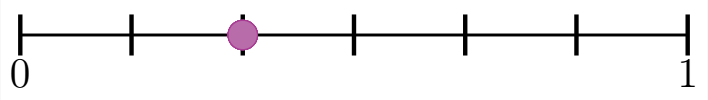
\includegraphics[width=150px]{../images/recta_num_frac01.png} \\[-0.5em] \fillin[$\dfrac{2}{6}$][2in]
			\part 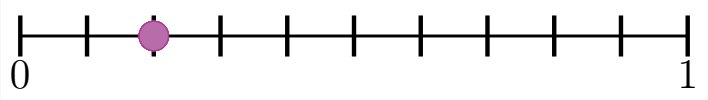
\includegraphics[width=150px]{../images/recta_num_frac02.png} \\[-0.5em] \fillin[$\dfrac{2}{10}$][2in]
			% \part 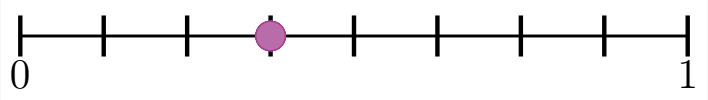
\includegraphics[width=150px]{../images/recta_num_frac03.png} \\[-0.5em] \fillin[$\dfrac{2}{6}$][1.5in]
			% \part 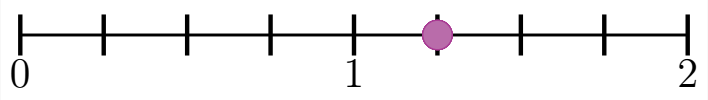
\includegraphics[width=150px]{../images/recta_num_frac04.png} \\[-0.5em] \fillin[$\dfrac{2}{6}$][1.5in]
			% \part 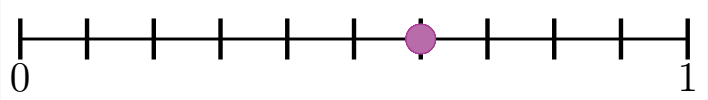
\includegraphics[width=150px]{../images/recta_num_frac05.png} \\[-0.5em] \fillin[$\dfrac{2}{6}$][1.5in]
			% \part 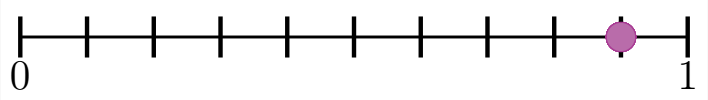
\includegraphics[width=150px]{../images/recta_num_frac06.png} \\[-0.5em] \fillin[$\dfrac{2}{6}$][1.5in]
			% \part 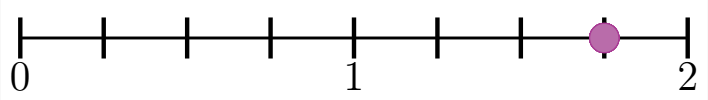
\includegraphics[width=150px]{../images/recta_num_frac07.png} \\[-0.5em] \fillin[$\dfrac{2}{6}$][1.5in]
			% \part 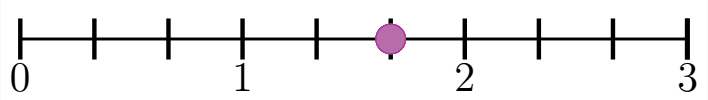
\includegraphics[width=150px]{../images/recta_num_frac08.png} \\[-0.5em] \fillin[$\dfrac{2}{6}$][1.5in]
			% \part 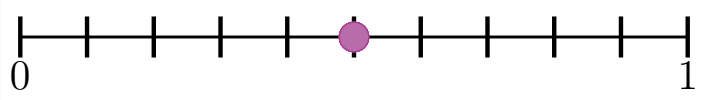
\includegraphics[width=150px]{../images/recta_num_frac09.png} \\[-0.5em] \fillin[$\dfrac{2}{6}$][1.5in]
			% \part 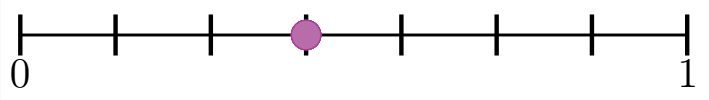
\includegraphics[width=150px]{../images/recta_num_frac10.png} \\[-0.5em] \fillin[$\dfrac{2}{6}$][1.5in]
		\end{parts}
	\end{multicols}
	}

      \questionboxed[2]{Escribe la fracción que representa el punto en la recta numérica
           
      \begin{multicols}{3}
                  \begin{parts}
                        \part 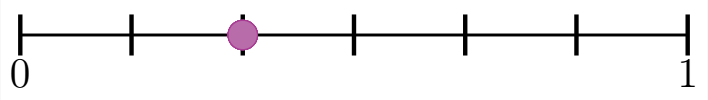
\includegraphics[width=\linewidth]{../images/recta_num_frac01.png} \\ \fillin[$\dfrac{2}{6}$][1in]
                        
						\part 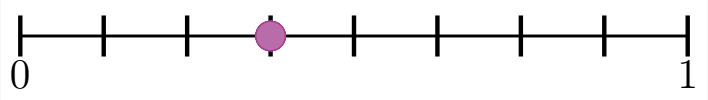
\includegraphics[width=\linewidth]{../images/recta_num_frac03.png} \\ \fillin[$\dfrac{3}{8}$][1in]
                        
						\part 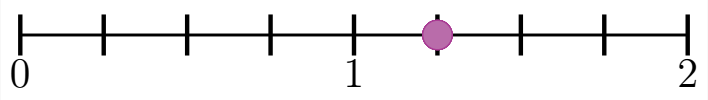
\includegraphics[width=\linewidth]{../images/recta_num_frac04.png} \\ \fillin[$\dfrac{5}{4}$][1in]
                        
						\part 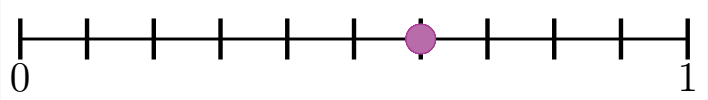
\includegraphics[width=\linewidth]{../images/recta_num_frac05.png} \\ \fillin[$\dfrac{6}{10}$][1in]
                        
						\part 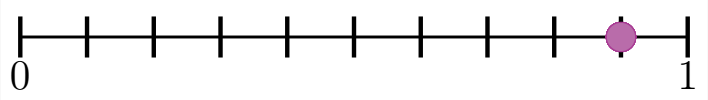
\includegraphics[width=\linewidth]{../images/recta_num_frac06.png} \\ \fillin[$\dfrac{9}{10}$][1in]
                        
						\part 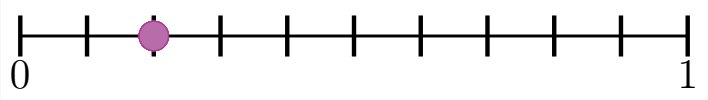
\includegraphics[width=\linewidth]{../images/recta_num_frac02.png} \\ \fillin[$\dfrac{2}{10}$][1in]
                        
						\part 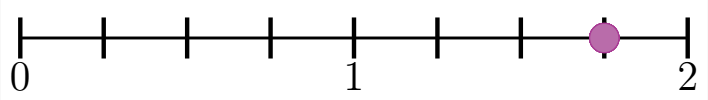
\includegraphics[width=\linewidth]{../images/recta_num_frac07.png} \\ \fillin[$\dfrac{7}{4}$][1in]
                        
						\part 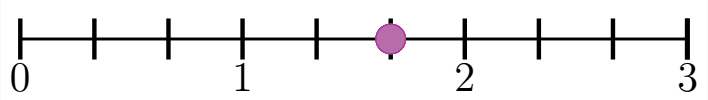
\includegraphics[width=\linewidth]{../images/recta_num_frac08.png} \\ \fillin[$\dfrac{5}{3}$][1in]
                        
						\part 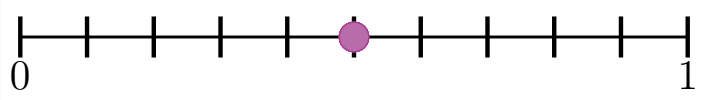
\includegraphics[width=\linewidth]{../images/recta_num_frac09.png} \\ \fillin[$\dfrac{5}{10}$][1in]
                        % \part 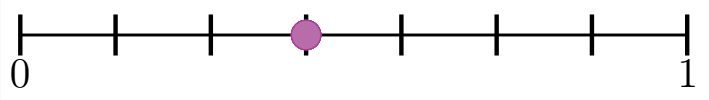
\includegraphics[width=\linewidth]{../images/recta_num_frac10.png} \\ \fillin[$\dfrac{3}{7}$][1in]
                  \end{parts}
            \end{multicols}
      }

      \subsubsection{Simplificación de fracciones}

	  	\ejemplosboxed[4]{Simplifica a su mínima expresión la siguiente fracción usando el máximo común divisor

	\begin{multicols}{2}
		\begin{parts}
			\part $\dfrac{8}{64}=$ \fillin[$\dfrac{1}{8}$][0in]
			\part $\dfrac{6}{42}=$ \fillin[$\dfrac{1}{7}$][0in]
		\end{parts}
	\end{multicols}
	}

	\questionboxed[4]{Simplifica a su mínima expresión la siguiente fracción usando el máximo común divisor
      
      \begin{multicols}{3}
                  \begin{parts}
                        \part $\dfrac{6}{42}=$ \fillin[$\dfrac{1}{7}$][0in]\\[1em]
						
                        \part $\dfrac{12}{18}=$ \fillin[$\dfrac{2}{3}$][0in]\\[1em]
						
                        \part $\dfrac{15}{30}=$ \fillin[$\dfrac{1}{2}$][0in]\\[1em]
						
                        \part $\dfrac{24}{36}=$ \fillin[$\dfrac{2}{3}$][0in]\\[1em]
						
                        \part $\dfrac{8}{64}=$ \fillin[$\dfrac{1}{8}$][0in]\\[1em]
						
                        \part $\dfrac{16}{24}=$ \fillin[$\dfrac{2}{3}$][0in]\\[1em]
						
                  \end{parts}
            \end{multicols}
      }

  \subsubsection{Fracciones equivalentes}
  
  \ejemplosboxed[4]{Indica si las siguientes fracciones son equivalentes o no:

	\begin{multicols}{2}
		\begin{parts}
			\part $\dfrac{2}{5}=\dfrac{8}{10}$\qquad
			\begin{oneparcheckboxes}
				\choice Sí
				\CorrectChoice No
			\end{oneparcheckboxes}

			\part $\dfrac{2}{8}=\dfrac{4}{16}$\qquad
			\begin{oneparcheckboxes}
				\CorrectChoice Sí
				\choice No
			\end{oneparcheckboxes}

			\part $\dfrac{1}{5}=\dfrac{5}{1}$\qquad
			\begin{oneparcheckboxes}
				\choice Sí
				\CorrectChoice No
			\end{oneparcheckboxes}

			\part $\dfrac{1}{10}=\dfrac{3}{30}$\qquad
			\begin{oneparcheckboxes}
				\CorrectChoice Sí
				\choice No
			\end{oneparcheckboxes}
		\end{parts}
	\end{multicols}
  }


  \questionboxed[3]{Indica si las siguientes fracciones son equivalentes o no:
  
  \begin{multicols}{2}
                  \begin{parts}
                        \part $\dfrac{4}{5}=\dfrac{8}{10}$\qquad
                        \begin{oneparcheckboxes}
                              \CorrectChoice Sí
                              \choice No
                        \end{oneparcheckboxes}

                        \part $\dfrac{1}{8}=\dfrac{4}{16}$\qquad
                        \begin{oneparcheckboxes}
                              \choice Sí
                              \CorrectChoice No
                        \end{oneparcheckboxes}

                        \part $\dfrac{1}{5}=\dfrac{5}{10}$\qquad
                        \begin{oneparcheckboxes}
                              \choice Sí
                              \CorrectChoice No
                        \end{oneparcheckboxes}

                        \part $\dfrac{1}{10}=\dfrac{3}{30}$\qquad
                        \begin{oneparcheckboxes}
                              \CorrectChoice Sí
                              \choice No
                        \end{oneparcheckboxes}

                        \part $\dfrac{1}{4}=\dfrac{2}{4}$\qquad
                        \begin{oneparcheckboxes}
                              \choice Sí
                              \CorrectChoice No
                        \end{oneparcheckboxes}

                        \part $\dfrac{3}{2}=\dfrac{12}{8}$\qquad
                        \begin{oneparcheckboxes}
                              \CorrectChoice Sí
                              \choice No
                        \end{oneparcheckboxes}

                        \part $\dfrac{3}{6}=\dfrac{1}{3}$\qquad
                        \begin{oneparcheckboxes}
                              \choice Sí
                              \CorrectChoice No
                        \end{oneparcheckboxes}

                        \part $\dfrac{18}{12}=\dfrac{9}{4}$\qquad
                        \begin{oneparcheckboxes}
                              \choice Sí
                              \CorrectChoice No
                        \end{oneparcheckboxes}
                  \end{parts}
            \end{multicols}
      }

%       \subsubsection{Comparación de fracciones}
     
% 	  	\ejemplosboxed[4]{Compara las siguientes fracciones usando los signos mayor que (>), menor que (<) o igual (=):

% 	\begin{multicols}{4}
% 		\begin{parts}
% 			\part $\dfrac{4}{3}$ \fillin[$>$][0.5in] $\dfrac{5}{4}$\\[0.75em]
% 			\part $\dfrac{1}{3}$ \fillin[$=$][0.5in] $\dfrac{3}{9}$\\[0.75em]
% 			% \part $\dfrac{2}{3}$ \fillin[$<$][0.5in] $\dfrac{3}{2}$\\[0.75em]
% 			% \part $\dfrac{3}{4}$ \fillin[$>$][0.5in] $\dfrac{2}{3}$\\[0.75em]
% 			\part $\dfrac{5}{6}$ \fillin[$>$][0.5in] $\dfrac{4}{5}$\\[0.75em]
% 			\part $\dfrac{1}{3}$ \fillin[$<$][0.5in] $\dfrac{2}{5}$\\[0.75em]
% 		\end{parts}
% 	\end{multicols}
% 	}

%       \questionboxed[4]{Compara las siguientes fracciones usando los signos mayor que (>), menor que (<) o igual (=):
         
%       \begin{multicols}{3}
%                   \begin{parts}
%                         % \part $\dfrac{2}{5}$ \fillin[$>$][0.5in] $\dfrac{1}{3}$\\[0.25em]
%                         \part $\dfrac{3}{4}$ \fillin[$<$][0.5in] $\dfrac{4}{5}$\\[0.25em]
                        
% 						\part $\dfrac{2}{5}$ \fillin[$<$][0.5in] $\dfrac{2}{3}$\\[0.25em]
                        
% 						\part $\dfrac{1}{5}$ \fillin[$<$][0.5in] $\dfrac{1}{4}$\\[0.25em]
                        
% 						\part $\dfrac{3}{2}$ \fillin[$=$][0.5in] $\dfrac{9}{6}$\\[0.25em]
                        
% 						\part $\dfrac{5}{6}$ \fillin[$>$][0.5in] $\dfrac{4}{6}$\\[0.25em]
                        
% 						\part $\dfrac{4}{3}$ \fillin[$>$][0.5in] $\dfrac{5}{4}$\\[0.25em]
                        
% 						\part $\dfrac{1}{3}$ \fillin[$=$][0.5in] $\dfrac{9}{3}$\\[0.25em]
                        
% 						\part $\dfrac{2}{3}$ \fillin[$<$][0.5in] $\dfrac{3}{2}$\\[0.25em]
%                         % \part $\dfrac{3}{5}$ \fillin[$>$][0.5in] $\dfrac{2}{3}$\\[0.25em]
                        
% 						\part $\dfrac{5}{6}$ \fillin[$>$][0.5in] $\dfrac{4}{5}$\\[0.25em]
%                   \end{parts}
%             \end{multicols}
%       }

%       \subsubsection{M.C.D y M.C.M}
   
% 	  \ejemplosboxed[4]{Calcula lo que se te pide en cada inciso:

% 	\begin{multicols}{2}
% 		\begin{parts}
% 			\part Encuentra el máximo común divisor de 120 y 300.

% 			\begin{solutionbox}{1cm}
% 				Se calcula el MCD$(120,300) = 60$.
% 			\end{solutionbox}

% \columnbreak%

% 			\part Encuentra el mínimo común múltiplo de 12, 15 y 18.

% 			\begin{solutionbox}{1cm}
% 				Se calcula el MCM$(12,15,18) = 180$.
% 			\end{solutionbox}

% 		\end{parts}
% 	\end{multicols}
% 	}

%       \questionboxed[4]{Calcula lo que se te pide en cada inciso:
    
%       \begin{multicols}{2}
%             \begin{parts}
%                   \part Encuentra el mínimo común múltiplo de 2 y 9.
              
%                   \begin{solutionbox}{2cm}
%                         El mínimo común múltiplo de 2 y 9 es 18.
%                   \end{solutionbox}

%                   \part Encuentra el máximo común divisor de 5 y 15.
            
%                   \begin{solutionbox}{2cm}
%                         El máximo común divisor de 5 y 15 es 5.
%                   \end{solutionbox}

%                   % \part Encuentra el mínimo común múltiplo de 2 y 5.
   
%                   % \begin{solutionbox}{1.2cm}
%                   %       El mínimo común múltiplo de 2 y 5 es 10.
%                   % \end{solutionbox}

%                   \part Encuentra el máximo común divisor de 33 y 121.
            
%                   \begin{solutionbox}{2cm}
%                         El máximo común divisor de 33 y 121 es 11.
%                   \end{solutionbox}

%                   \part Encuentra el máximo común divisor de 25 y 100.
             
%                   \begin{solutionbox}{2cm}
%                         El máximo común divisor de 25 y 100 es 25.
%                   \end{solutionbox}

%                   \part Encuentra el máximo común divisor de 18 y 36.
              
%                   \begin{solutionbox}{2cm}
%                         El máximo común divisor de 18 y 36 es 18.
%                   \end{solutionbox}

%                   % \part Encuentra el mínimo común múltiplo de 4 y 9.
               
%                   % \begin{solutionbox}{1.2cm}
%                   %       El mínimo común múltiplo de 4 y 9 es 36.
%                   % \end{solutionbox}

%                   % \part Encuentra el mínimo común múltiplo de 6 y 7.
                
%                   % \begin{solutionbox}{1.2cm}
%                   %       El mínimo común múltiplo de 6 y 7 es 42.
%                   % \end{solutionbox}

%                   \part Encuentra el mínimo común múltiplo de 2, 3 y 4.
                 
%                   \begin{solutionbox}{1.2cm}
%                         El mínimo común múltiplo de 2, 3 y 4 es 12.
%                   \end{solutionbox}

%                   \part Encuentra el máximo común divisor de 2 y 14.
                  
%                   \begin{solutionbox}{1.2cm}
%                         El máximo común divisor de 2 y 14 es 2.
%                   \end{solutionbox}
            
%                   \part Encuentra el mínimo común múltiplo de 12, 15 y 18.
                 
%                   \begin{solutionbox}{1.2cm}
%                         El mínimo común múltiplo de 12, 15 y 18 es 180.
%                   \end{solutionbox}
%             \end{parts}
%       \end{multicols}
%       }

%       \subsubsection{Resolución de problemas}

% 	    \ejemplosboxed[2]{María y Jorge tienen 24 bolas blancas, 40 bolas azules y 72 bolas rojas y quieren hacer el mayor número de collares iguales sin que sobre ninguna bola. ¿Cuántos collares iguales pueden hacer?
         
%       \begin{solutionbox}{2cm}
%                   Se calcula el M.C.D.$(24,40,72) = 8$.\\
%                   Por lo tanto, se pueden hacer 8 collares.
%             \end{solutionbox}
%       }

%       \questionboxed[3]{María y Jorge tienen 45 bolas blancas, 15 bolas azules y 90 bolas rojas y quieren hacer el mayor número de collares iguales sin que sobre ninguna bola. ¿Cuántos collares iguales pueden hacer?
         
%       \begin{solutionbox}{2cm}
%                   Se calcula el M.C.D.$(45,15,90) = 15$.\\
%                   Por lo tanto, se pueden hacer 15 collares.
%             \end{solutionbox}
%       }

	\subsection{Operaciones con fracciones}
	
\ejemplosboxed[6]{Realiza las siguientes operaciones con fracciones (simplifica el resultado a la mínima expresión):

    \begin{multicols}{3}

        \begin{parts}\large
				\subsubsection{Suma y resta con denominadores iguales}

            \part $\dfrac{7}{8}-\dfrac{3}{8}=$ \fillin[$\dfrac{4}{8}=\dfrac{1}{2}$][0in]\\[0.5em]
	
			\subsubsection{Multiplicación de fracciones}

            \part $\dfrac{9}{5}\times\dfrac{15}{4}=$ \fillin[$\dfrac{135}{20}=\dfrac{27}{4}$][0in]\\[0.5em]
          
			\columnbreak%

				\subsubsection{Suma y resta denominadores diferentes}

            \part $\dfrac{7}{8}-\dfrac{3}{7}=$ \fillin[$\dfrac{49}{56}-\dfrac{24}{56}=\dfrac{25}{56}$][0in] \\[3em]

            \part $\dfrac{5}{8}+\dfrac{3}{4}=$ \fillin[$\dfrac{5}{8}+\dfrac{6}{8}=\dfrac{11}{8}$][0in]  \\[3em]
              	
			\columnbreak%

			\subsubsection{División de fracciones}
			
            \part $\dfrac{3}{5} \divisionsymbol\dfrac{2}{3}=$ \fillin[$\dfrac{9}{10}$][0in]  \\[1em]

            \part $\dfrac{7}{12}\divisionsymbol\dfrac{2}{3}=$ \fillin[$\dfrac{21}{24}=\dfrac{7}{8}$][0in]\\[1em]

        \end{parts}
    \end{multicols}
	}

	% \subsubsection{Suma y resta con denominadores iguales}

	\questionboxed[3]{ Realiza las siguientes sumas y restas de fracciones con denominadores iguales:
		\begin{multicols}{3}
			\begin{parts}\large
				\part $\dfrac{3}{5}+\dfrac{2}{5}=$ \fillin[$\dfrac{5}{5}=1$][0in]\\[1em]
				\part $\dfrac{7}{8}-\dfrac{3}{8}=$ \fillin[$\dfrac{5}{8}$][0in]\\[1em]
				\part $\dfrac{37}{12}-\dfrac{11}{12}=$ \fillin[$\dfrac{13}{6}=1$][0in]\\[1em]
				% \part $\dfrac{7}{4}+\dfrac{3}{4}=$ \fillin[$\dfrac{}{}+\dfrac{}{}=\dfrac{}{}$][0in]\\[1em]
				% \part $\dfrac{1}{3}+\dfrac{2}{3}=$ \fillin[$\dfrac{}{}+\dfrac{}{}=\dfrac{}{}$][0in]\\[1em]
				% \part $\dfrac{5}{4}+\dfrac{8}{4}=$ \fillin[$\dfrac{}{}+\dfrac{}{}=\dfrac{}{}$][0in]\\[1em]
			\end{parts}
		\end{multicols}
	}

	% \subsubsection{Suma y resta denominadores diferentes}
	\questionboxed[3]{ Realiza las siguientes sumas y restas de fracciones con denominadores diferentes:
		\begin{multicols}{3}
			\begin{parts}\large
				\part $\dfrac{3}{5}+\dfrac{2}{3}=$ \fillin[$\dfrac{9}{15}+\dfrac{10}{15}=\dfrac{19}{15}$][0in]\\[1em]
				\part $\dfrac{7}{8}+\dfrac{3}{4}=$ \fillin[$\dfrac{7}{8}+\dfrac{6}{8}=\dfrac{13}{8}$][0in]\\[1em]
				\part $\dfrac{2}{3}-\dfrac{1}{6}=$ \fillin[$\dfrac{2}{3}-\dfrac{1}{6} =\dfrac{1}{2}$][0in]\\[1em]
				\part $\dfrac{5}{6}-\dfrac{3}{8}=$ \fillin[$\dfrac{5}{6}-\dfrac{3}{8} =\dfrac{11}{24}$][0in]\\[1em]
				\part $\dfrac{4}{5}-\dfrac{3}{10}=$ \fillin[$\dfrac{4}{5}-\dfrac{3}{10} =\dfrac{1}{2}$][0in]\\[1em]
				\part $\dfrac{1}{3}-\dfrac{1}{5}=$ \fillin[$\dfrac{1}{3}-\dfrac{1}{5} = \dfrac{2}{5}$][0in]\\[1em]
			\end{parts}
		\end{multicols}
	}

	% \subsubsection{Multiplicación de fracciones}
	\questionboxed[6]{ Realiza las siguientes multiplicaciones de fracciones:
		
	\begin{multicols}{3}
			\begin{parts}\large
				\part $\dfrac{3}{5}\times\dfrac{2}{3}=$ \fillin[$\dfrac{6}{15}$][0in]\\[1em]
				\part $\dfrac{7}{8}\times\dfrac{3}{4}=$ \fillin[$\dfrac{21}{32}$][0in]
				
				\columnbreak%

				\part $5\times\dfrac{7}{3}=$ \fillin[$\dfrac{4}{9}\times 2=\dfrac{8}{9}$][0in]\\[1em]
				\part $\dfrac{4}{9}\times 2=$ \fillin[$\dfrac{4}{9}\times 2=\dfrac{8}{9}$][0in]

				\columnbreak%

			\part $\dfrac{4}{3}\times\dfrac{7}{8}=$ \fillin[$\dfrac{4}{3}\times\dfrac{7}{8}=\dfrac{7}{6}$][0in]\\[1em]
			\part $\dfrac{9}{5}\times\dfrac{15}{4}=$ \fillin[$\dfrac{9}{5}\times\dfrac{15}{4}=\dfrac{27}{4}$][0in]
        \end{parts}
		\end{multicols}
	}

	% \subsubsection{División de fracciones}
	\questionboxed[2]{ Realiza las siguientes divisiones de fracciones:

		\begin{multicols}{2}
			\begin{parts}\large
				\part $ \dfrac{3}{4} \divisionsymbol\dfrac{2}{5}=$ \fillin[$\dfrac{15}{8}$][0in]

				\part $ \dfrac{7}{12}\divisionsymbol\dfrac{2}{3}=$ \fillin[$\dfrac{7}{8}$][0in]
            \end{parts}
		\end{multicols}
	}

	\subsubsection{Resolución de problemas}

	  \ejemplosboxed[10]{Resuelve los siguientes problemas:

    \begin{parts}
        \part Un granjero siembra 3/5 de su granja con maíz y 1/8 con soya, ¿qué cantidad de su granja queda por sembrar?

        \begin{solutionbox}{1.8cm}
            Para conocer la cantidad de su granja que queda por sembrar, se debe restar 3/5 y 1/8 a 1; entonces:
            \[1-\dfrac{3}{5}-\dfrac{1}{8}=\dfrac{40}{40}-\dfrac{24}{40}-\dfrac{5}{40}=\dfrac{11}{40}\]

        \end{solutionbox}

        % \part Un reloj se adelanta 3/7 de minuto cada hora. ¿Cuánto se adelantará en 5 horas?

        % \begin{solutionbox}{2.5cm}
        %     Para conocer cuánto se adelantará en 5 horas, se debe multiplicar 3/7 por 5; entonces:
        %     \[\dfrac{3}{7}\times 5=\dfrac{15}{7}\]
        % \end{solutionbox}
    \end{parts}
	  }

	\questionboxed[4]{ Resuelve los siguientes problemas:
		\begin{parts}
			\part Un granjero siembra 2/5 de su granja con maíz y 3/10 con soya, ¿qué cantidad de su granja queda por sembrar?
			\begin{solutionbox}{1.8cm}
				Para conocer la cantidad de su granja que queda por sembrar, se debe restar 2/5 y 3/10 a 1; entonces:
				\[1-\dfrac{2}{5}-\dfrac{3}{10}=\dfrac{10}{10}-\dfrac{4}{10}-\dfrac{3}{10}=\dfrac{3}{10}\]

			\end{solutionbox}

			\part Un reloj se adelanta 3/7 de minuto cada hora. ¿Cuánto se adelantará en 5 horas?
			\begin{solutionbox}{1.8cm}
				Para conocer cuánto se adelantará en 5 horas, se debe multiplicar 3/7 por 5; entonces:
				\[\dfrac{3}{7}\times 5=\dfrac{15}{7}\]
			\end{solutionbox}
		\end{parts}
	}


      \subsection{Números negativos}
     
      \subsubsection{Determina el signo}
     
	  \ejemplosboxed[4]{Determina el signo \textit{positivo} o \textit{negativo} que resulta de las siguientes operaciones:

	\begin{multicols}{2}
		\begin{parts}\normalsize
			\part $-28-19$ \fillin[Negativo][1in]
			\part $-43+55$ \fillin[Positivo][1in]
		\end{parts}
	\end{multicols}
	}


      \questionboxed[4]{Determina el signo \textit{positivo} o \textit{negativo} que resulta de las siguientes operaciones:
          
      \begin{multicols}{2}
                  \begin{parts}
                        \part $-28-19$ \fillin[Negativo][1in]\\
                        \part $-43+55$ \fillin[Positivo][1in]\\
                        \part $-223-67$ \fillin[Negativo][1in]\\
                        \part $-23+81$ \fillin[Positivo][1in]
                        \part $74-67$ \fillin[Positivo][1in]\\
                        \part $44-80$ \fillin[Negativo][1in]\\
                        \part $87-67$ \fillin[Positivo][1in]\\
                        \part $-105+95$ \fillin[Negativo][1in]
                  \end{parts}
                  \end{multicols}
      }

      \subsubsection{Suma y resta con negativos}
    
 \ejemplosboxed[8]{Realiza las siguientes operaciones con números negativos:
          
      \begin{multicols}{3}
                  \begin{parts}
                        \part $28-19=$ \fillin[$9$][0in]\\
                        \part $-43-45=$ \fillin[$-98$][0in]
                        \part $23-32=$ \fillin[$-9$][0in]\\
                        \part $-5+7=$ \fillin[$2$][0in]
                         \part $-90+25=$  \fillin[$-65$][0in]\\
                        \part $-16-9=$  \fillin[$-25$][0in]
                  \end{parts}
            \end{multicols}
      }      
      

      \questionboxed[8]{Realiza las siguientes operaciones con números negativos:
          
      \begin{multicols}{3}
                  \begin{parts}
                        \part $-28+19=$ \fillin[$-9$][0in]\\
                        \part $-43-55=$ \fillin[$-98$][0in]\\
                        \part $-223+67=$ \fillin[$-156$][0in]\\
                        \part $-23+67=$ \fillin[$44$][0in]
                         \part $-90+25=$  \fillin[$-65$][0in]\\
                        \part $-16-99=$  \fillin[$-115$][0in]\\
                        % \part $-137-350=$ \fillin[$-487$][0in]
                        % \part $203-661=$    \fillin[$-458$][0in]
                        \part $-223+67=$ \fillin[$-156$][0in]\\
                        \part $-68+29=$ \fillin[$-39$][0in]
                        \part $-416-90=$ \fillin[$-506$][0in]\\
                        \part $-64-94=$ \fillin[$-158$][0in]\\
                        \part $-91-209=$ \fillin[$-300$][0in]\\
                        \part $12-107=$ \fillin[$-95$][0in]
                  \end{parts}
            \end{multicols}
      }      
      
      \subsubsection{Ubicación en la recta numérica}
     
	  \ejemplosboxed[4]{Escribe el número que representa el punto indicado en la recta numérica de cada uno de los siguientes incisos.

	\begin{multicols}{3}
		\begin{parts}
                        \part 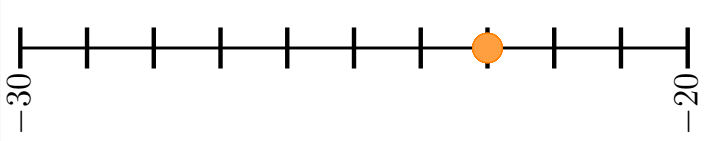
\includegraphics[width=0.8\linewidth]{../images/recta_num_-23.png}  \\[-1em]  \fillin[$-23$][1.5in]
                        \part 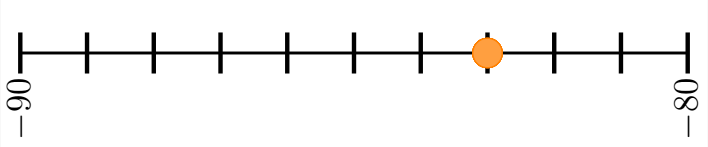
\includegraphics[width=0.8\linewidth]{../images/recta_num_-83.png}  \\[-1em]  \fillin[$-83$][1.5in]
                        \part 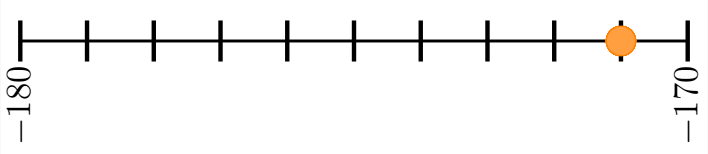
\includegraphics[width=0.8\linewidth]{../images/recta_num_-171.png} \\[-1em]   \fillin[$-171$][1.5in] 
		\end{parts}
	\end{multicols}
	}

      \questionboxed[4]{Escribe el número que representa el punto indicado en la recta numérica de cada uno de los siguientes incisos.

            \begin{multicols}{3}
                  \begin{parts}
                        \part 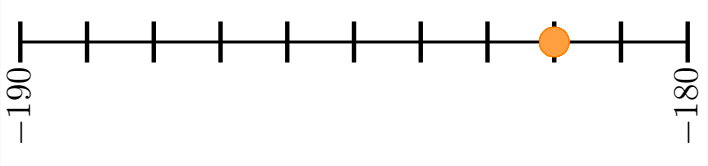
\includegraphics[width=0.8\linewidth]{../images/recta_num_-182.png} \\[-1em]   \fillin[$-182$][1.5in]
                        \part 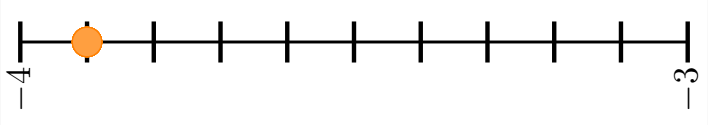
\includegraphics[width=0.8\linewidth]{../images/recta_num_-3.9.png} \\[-1em]  \fillin[$-3.9$][1.5in]
                        \part 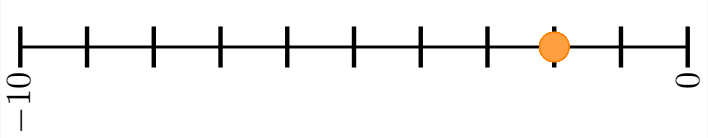
\includegraphics[width=0.8\linewidth]{../images/recta_num_-2.png}   \\[-1em]  \fillin[$-2$][1.5in]
                        \part 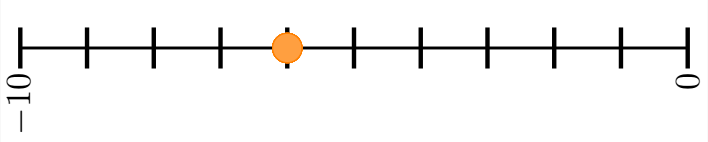
\includegraphics[width=0.8\linewidth]{../images/recta_num_-6.png}   \\[-1em]  \fillin[$-6$][1.5in]
                        \part 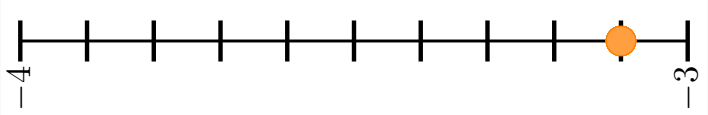
\includegraphics[width=0.8\linewidth]{../images/recta_num_-3.1.png} \\[-1em]   \fillin[$-3.1$][1.5in] 
                        \part 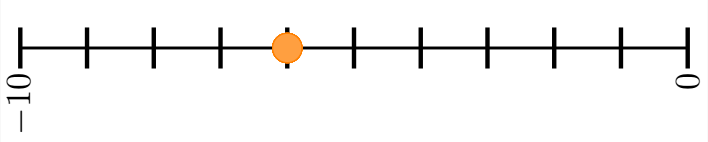
\includegraphics[width=0.8\linewidth]{../images/recta_num_-6.png}   \\[-1em] \fillin[$-6$][1.5in]     
                  \end{parts}
            \end{multicols}
      }

	  \ejemplosboxed[6]{Realiza las siguientes operaciones con números negativos:

	\begin{multicols}{3}
		\begin{parts}\normalsize
			\part $-223+67=$ \fillin[$-156$][0in]
			\part $(16)-(-14)=$ \fillin[$30$][0in]
			\part $(-16)+(-81)=$ \fillin[$-97$][0in]
		\end{parts}
	\end{multicols}
	}

      \questionboxed[8]{Realiza las siguientes operaciones de acuerdo con la jerarquía de operaciones:
           
      \begin{multicols}{3}
                  \begin{parts}\normalsize
                        \part $(64)-(-231)+(87)=$ \fillin[$382$][0in]
                        
						\part $(-16)+(-81)=$ \fillin[$-97$][0in]
                        
						\part $(121)-(54)+(-14)=$ \fillin[$53$][0in]
                        
						\part $(-13)-(91)=$ \fillin[$-104$][0in]
                        
						\part $(-97)+(55)=$ \fillin[$-42$][0in]
                        
						\part $(54)+(-97)+(-71)=$ \fillin[$-114$][0in]
                        
						\part $(57)+(-211)-(-81)=$ \fillin[$-73$][0in]
                        
						\part $(134)-(-94)=$ \fillin[$228$][0in]
                        
						\part $(16)-(-14)$ \fillin[$30$][0in]
                        
						\part $-23-(-67)$ \fillin[$44$][0in]
                        
						\part $-74-(-67)$ \fillin[$-7$][0in]
                        
						\part $-44-(-80)$ \fillin[$36$][0in]
                  \end{parts}
            \end{multicols}
      }

      \subsubsection{Comparación de negativos}
   
	  \ejemplosboxed[4]{Escribe sobre la línea el símbolo de mayor que ($>$), menor que ($<$), o igual ($=$) según corresponda.

	\begin{multicols}{2}
		\begin{parts}\normalsize
			\part $-182$ \fillin[$>$][0.5in] $-189$
			% \part $-97$ \fillin[$<$][0.5in] $-96.2$
			\part $-51$ \fillin[$>$][0.5in] $-55$\\[0.1em]
		\end{parts}
	\end{multicols}
	}

      \questionboxed[4]{Escribe sobre la línea el símbolo de mayor que ($>$), menor que ($<$), o igual ($=$) según corresponda.
      
      \begin{multicols}{3}
                  \begin{parts}
                        \part $-59$ \fillin[$<$][0.5in] $-55$\\[0.1em]
                        % \part $-77$ \fillin[$>$][0.5in] $-177$\\[0.1em]
                        \part $-100$ \fillin[$<$][0.5in] $-99$\\[0.1em]
                        \part $-192$ \fillin[$<$][0.5in] $-189$\\[0.1em]
                        \part $-97$ \fillin[$<$][0.5in] $-96$\\[0.1em]
                        \part $-36$ \fillin[$>$][0.5in] $-39$\\[0.1em]
                        % \part $-3.5$ \fillin[$<$][0.5in] $-2.2$\\[0.1em]
                        \part $-12$ \fillin[$<$][0.5in] $-11$\\[0.1em]
                        % \part $-10.001$ \fillin[$>$][0.5in] $-100.01$\\[0.1em]
                        % \part $-0.99$ \fillin[$>$][0.5in] $1.01$\\[0.1em]
                        % \part $-3.9$ \fillin[$>$][0.5in] $-4.1$\\[0.1em]
                        % \part $-0.5$ \fillin[$<$][0.5in] $-0.4$\\[0.1em]
                        % \part $-1.2$ \fillin[$<$][0.5in] $-1.02$\\[0.1em]
                        % \part $-0.5$ \fillin[$>$][0.5in] $-0.6$\\[0.1em]
                  \end{parts}
            \end{multicols}
      }

      % \addcontentsline{toc}{subsection}{Jerarquía de operaciones}
	\subsubsection{Jerarquía de operaciones}
  
    \ejemplosboxed[4]{Usando la jerarquía de operaciones, realiza la siguiente operación

            \begin{multicols}{2}
                  \begin{parts}
                        % \part $9+6\times 4-5=$ \fillin[$28$][0in]
                        \part $7+2^2 \times 6+2^2-6=$ \fillin[$29$][0in]
                        \part $10\times 12-14\divisionsymbol 2+15=$ \fillin[$128$][0in]
                        % \part $6^3 \divisionsymbol 8 \divisionsymbol 9 = $ \fillin[$3$][0in]
                        % \part $8\times 3 +70\divisionsymbol 7-7=$ \fillin[$27$][0in]
                        % \part $16 \times 15 \divisionsymbol 5 +12=$ \fillin[$60$][0in]
                  \end{parts}
            \end{multicols}
      }


      \questionboxed[4]{Usando la jerarquía de operaciones, realiza la siguiente operación

            \begin{multicols}{2}
                  \begin{parts}
                        % \part $9+6\times 4-5=$ \fillin[$28$][0in]
                        % \part $7+2^2 \times 6+2^2-6=$ \fillin[$29$][0in]
                        % \part $10\times 12-14\divisionsymbol 2+15=$ \fillin[$128$][0in]
                        \part $6^3 \divisionsymbol 8 \divisionsymbol 9 = $ \fillin[$3$][0in]
                        \part $8\times 3 +70\divisionsymbol 7-7=$ \fillin[$27$][0in]
                        \part $16 \times 15 \divisionsymbol 5 +12=$ \fillin[$60$][0in]
                  \end{parts}
            \end{multicols}
      }

      % \addcontentsline{toc}{section}{Sucesiones aritméticas}
	\subsection{Sucesiones aritméticas}
   
      % \addcontentsline{toc}{subsection}{Completando la sucesión}
	\subsubsection{Completando la sucesión}
    
        \ejemplosboxed[2]{Escribe los términos faltantes de las siguientes sucesiones aritméticas:
         
      \begin{multicols}{2}
                  \begin{parts}
                        \part $ -7,-13,-18,$\fillin[$-23$][0.3in],\fillin[$-28$][0.3in],\fillin[$-33$][0.3in],\ldots
                        \part $-59,-65,-71,$\fillin[$-77$][0.3in],\fillin[$-83$][0.3in],\fillin[$-89$][0.3in],\ldots
                        \part $14,17,20,$\fillin[$23$][0.3in],\fillin[$26$][0.3in],\fillin[$29$][0.3in],\ldots
                        \part $19,23,27,$\fillin[$31$][0.3in],\fillin[$35$][0.3in],\fillin[$39$][0.3in],\ldots
                  \end{parts}
            \end{multicols}
      }

      
      \questionboxed[2]{Escribe los términos faltantes de las siguientes sucesiones aritméticas:
         
      \begin{multicols}{2}
                  \begin{parts}
                        \part $ -8,-13,-18,$\fillin[$-23$][0.3in],\fillin[$-28$][0.3in],\fillin[$-33$][0.3in],\ldots
                        \part $-57,-65,-73,$\fillin[$-81$][0.3in],\fillin[$-89$][0.3in],\fillin[$-97$][0.3in],\ldots
                        \part $-14,-17,-20,$\fillin[$-23$][0.3in],\fillin[$-26$][0.3in],\fillin[$-29$][0.3in],\ldots
                        \part $-19,-15,-11,$\fillin[$-7$][0.3in],\fillin[$-3$][0.3in],\fillin[$1$][0.3in],\ldots
                  \end{parts}
            \end{multicols}
      }

      % \addcontentsline{toc}{subsection}{Diferencia de una sucesión}
	\subsubsection{Diferencia de una sucesión}
   
\ejemplosboxed[2]{Determina la diferencia de las siguientes sucesiones aritméticas:
           
      \begin{multicols}{2}
                  \begin{parts}
                        \part $-63,-58,-53,-48,-43,\ldots$ \hfill d=\fillin[$5$][1cm]
                        \part $-1,-4,-7,-10,-13,\ldots$ \hfill d=\fillin[$-3$][1cm]
                        \part $8,4,0,-4,-8,\ldots$ \hfill d=\fillin[$-4$][1cm]
                        \part $-11,1,13,\ldots$ \hfill d=\fillin[$12$][1cm]
                  \end{parts}
            \end{multicols}
      }

      \questionboxed[2]{Determina la diferencia de las siguientes sucesiones aritméticas:
           
      \begin{multicols}{2}
                  \begin{parts}
                        \part $-23,-15,-7,1,9,17,\ldots$ \hfill d=\fillin[$8$][1cm]\\
                        \part $-15,-10,-5,0,5,\ldots$ \hfill d=\fillin[$5$][1cm]\\
                        \part $-8,-13,-18,-23,-28,-33,\ldots$ \hfill d=\fillin[$-5$][1cm]\\
                        \part $-19,-15,-11,-7,-3,1,\ldots$ \hfill d=\fillin[$4$][1cm]\\
                        \part $7,9,11,13,15,17,\ldots$ \hfill d=\fillin[$2$][1cm]\\
                        \part $-4,-2,0,2,4,6,\ldots$ \hfill d=\fillin[$2$][1cm]\\
                  \end{parts}
            \end{multicols}
      }

      % \addcontentsline{toc}{subsection}{Término enésimo}
	\subsubsection{Término enésimo}
 
       \ejemplosboxed[4]{Encuentra el \textit{n-ésimo} término de la siguientes sucesiones aritméticas:
           
      \begin{multicols}{2}
                  \begin{parts}
                        \part Calcula el término número 44 de la siguiente sucesión aritmética: $-3n-15$
                       
                        \begin{solutionbox}{0.8cm}
                             $-3(44)-15=-132-15=-147$
                        \end{solutionbox}

                        \part Calcula el término número 47 de la siguiente sucesión aritmética: $-5,0,5,10,15,\ldots$
                       
                        \begin{solutionbox}{0.8cm}
                             $5(47)=235$
                        \end{solutionbox}

                        % \part Calcula el término número 28 de la siguiente sucesión aritmética: $-69,-72,-75,-78,-81,\ldots$
                       
                        % \begin{solutionbox}{1cm}
                        %      $-3(28)-66=-84-66=-150$
                        % \end{solutionbox}

                        % \part Calcula el término número 15 de la siguiente sucesión aritmetica: $11,18,25,32,39,\ldots$
                       
                        % \begin{solutionbox}{1cm}
                        %      $7(15)+4=105+4=109$
                        % \end{solutionbox}

                        % \part Calcula el término número 25 de la siguiente sucesión aritmética: $2n-6$
                       
                        % \begin{solutionbox}{1cm}
                        %      $2(25)-6=50-6=44$
                        % \end{solutionbox}

                        % \part Calcula el término número 22 de la siguiente sucesión aritmética: $7,2,-3,-8,-13,\ldots$
                     
                        % \begin{solutionbox}{1cm}
                        %      $-5(22)+12=-110+12=-98$
                        % \end{solutionbox}
                  \end{parts}
            \end{multicols}
      }

      \questionboxed[4]{Encuentra el \textit{n-ésimo} término de la siguientes sucesiones aritméticas:
           
      \begin{multicols}{2}
                  \begin{parts}
                        % \part Calcula el término número 44 de la siguiente sucesión aritmética: $-3n-15$
                       
                        % \begin{solutionbox}{1cm}
                        %      $-3(44)-15=-132-15=-147$
                        % \end{solutionbox}

                        % \part Calcula el término número 47 de la siguiente sucesión aritmética: $-5,0,5,10,15,\ldots$
                       
                        % \begin{solutionbox}{1cm}
                        %      $5(47)=235$
                        % \end{solutionbox}

                        \part Calcula el término número 28 de la siguiente sucesión aritmética: $-69,-72,-75,-78,-81,\ldots$
                       
                        \begin{solutionbox}{1cm}
                             $-3(28)-66=-84-66=-150$
                        \end{solutionbox}

                        \part Calcula el término número 15 de la siguiente sucesión aritmetica: $11,18,25,32,39,\ldots$
                       
                        \begin{solutionbox}{1cm}
                             $7(15)+4=105+4=109$
                        \end{solutionbox}

                        \part Calcula el término número 25 de la siguiente sucesión aritmética: $2n-6$
                       
                        \begin{solutionbox}{1cm}
                             $2(25)-6=50-6=44$
                        \end{solutionbox}

                        \part Calcula el término número 22 de la siguiente sucesión aritmética: $7,2,-3,-8,-13,\ldots$
                     
                        \begin{solutionbox}{1cm}
                             $-5(22)+12=-110+12=-98$
                        \end{solutionbox}
                  \end{parts}
            \end{multicols}
      }
      
      % \addcontentsline{toc}{subsection}{Término general}
	\subsubsection{Término general}
 
 \ejemplosboxed[4]{Determina el término general de las siguientes sucesiones aritméticas:
           
      \begin{multicols}{2}
                  \begin{parts}
                        \part $3,9,15,21,27,\ldots$ \fillin[$6n-3$][1in]
                        \part $-69,-72,-75,-78,-81,\ldots$ \fillin[$-3n-66$][1in]
                        % \part $40,35,30,25,20,\ldots$ \fillin[$5-5n$][1in]
                        % \part $-2,-6,-10,-14,-18,\ldots$ \fillin[$-4n+2$][1in]
                        % \part $-2,1,4,7,10,\ldots$ \fillin[$3n-5$][1in]
                        % \part $-57,-65,-73,-81,-89,\ldots$ \fillin[$-8n-49$][1in]
                  \end{parts}
            \end{multicols}
      }

      \questionboxed[4]{Determina el término general de las siguientes sucesiones aritméticas:
           
      \begin{multicols}{2}
                  \begin{parts}
                        % \part $3,9,15,21,27,\ldots$ \fillin[$6n-3$][1in]
                        % \part $-69,-72,-75,-78,-81,\ldots$ \fillin[$-3n-66$][1in]
                        \part $40,35,30,25,20,\ldots$ \fillin[$5-5n$][1in]
                        \part $-2,-6,-10,-14,-18,\ldots$ \fillin[$-4n+2$][1in]
                        \part $-2,1,4,7,10,\ldots$ \fillin[$3n-5$][1in]
                        \part $-57,-65,-73,-81,-89,\ldots$ \fillin[$-8n-49$][1in]
                  \end{parts}
            \end{multicols}
      }

      % \addcontentsline{toc}{subsection}{Suma de una sucesión aritmética}
	\subsubsection{Suma de una sucesión aritmética}

        \ejemplosboxed[6]{Resuelve las siguientes \emph{sumas} de sucesiones aritméticas:
       
      % \begin{multicols}{2}
                  \begin{parts}
                        \part Calcula la suma de los primeros 41 términos de la siguiente sucesión aritmética: $40,51,62,73,84,\ldots$
                       
                        \begin{solutionbox}{1cm}
                              $a_{41}=40+11(41-1)=40+440=480$ \qquad
                              $S_{41}=\dfrac{41(40+480)}{2}=10,660$
                        \end{solutionbox}

                        \part Calcula la suma de los primeros 37 términos de la siguiente sucesión aritmética: $15,25,35,45,55,\ldots$
                        
                        \begin{solutionbox}{1cm}
                              $a_{37}=15+10(37-1)=15+360=375$ \qquad
                              $S_{37}=\dfrac{37(15+375)}{2}=7,215$
                        \end{solutionbox}

                        % \part Calcula la suma de los primeros 23 términos de la siguiente sucesión aritmética: $-5,0,5,10,15,\ldots$
                       
                        % \begin{solutionbox}{2cm}
                        %       \[a_{23}=-5+5(23-1)=-5+110=105\]
                        %       \[S_{23}=\dfrac{23(-5+105)}{2}=1,150\]
                        % \end{solutionbox}

                        % \part Calcula la suma de los primeros 25 términos de la siguiente sucesión aritmética: $11,18,25,32,39,\ldots$
                      
                        % \begin{solutionbox}{2cm}
                        %       \[a_{25}=11+7(25-1)=11+168=179\]
                        %       \[S_{25}=\dfrac{25(11+179)}{2}=2,375\]
                        % \end{solutionbox}
                  \end{parts}
            % \end{multicols}
      }

      \questionboxed[8]{Calcula la suma de los primeros $n$ términos de las siguientes sucesiones aritméticas:
       
      % \begin{multicols}{2}
                  \begin{parts}
                        % \part Calcula la suma de los primeros 41 términos de la siguiente sucesión aritmética: $40,51,62,73,84,\ldots$
                       
                        % \begin{solutionbox}{2cm}
                        %       \[a_{41}=40+11(41-1)=40+440=480\]
                        %       \[S_{41}=\dfrac{41(40+480)}{2}=10,660\]
                        % \end{solutionbox}

                        % \part Calcula la suma de los primeros 37 términos de la siguiente sucesión aritmética: $15,25,35,45,55,\ldots$
                        
                        % \begin{solutionbox}{2cm}
                        %       \[a_{37}=15+10(37-1)=15+360=375\]
                        %       \[S_{37}=\dfrac{37(15+375)}{2}=7,215\]
                        % \end{solutionbox}

                        \part Calcula la suma de los primeros 23 términos de la siguiente sucesión aritmética: $-5,0,5,10,15,\ldots$
                       
                        \begin{solutionbox}{2cm}
                              \[a_{23}=-5+5(23-1)=-5+110=105\]
                              \[S_{23}=\dfrac{23(-5+105)}{2}=1,150\]
                        \end{solutionbox}

                        \part Calcula la suma de los primeros 25 términos de la siguiente sucesión aritmética: $11,18,25,32,39,\ldots$
                      
                        \begin{solutionbox}{2cm}
                              \[a_{25}=11+7(25-1)=11+168=179\]
                              \[S_{25}=\dfrac{25(11+179)}{2}=2,375\]
                        \end{solutionbox}
                  \end{parts}
            % \end{multicols}
      }